\subsubsection{Naming engine}

The naming engine turned out to be one of the most complex parts of the project. The naming engine is responsible for checking the names of various parts of the codebase, such as classes, methods, and variables and then converting them to match the user-defined configuration. The naming engine is split into multiple modules: the diagnostic module, code fix module; and the regex engine module. The diagnostic module is responsible for finding the issues in the codebase, the code fix module is responsible for fixing the issues, and the regex engine module is responsible for converting the names to match the user-defined configuration.

The diagnostic module uses the Roslyn API to parse the codebase and analyze objects, classes, methods, and variables. In order to reliably verify a name, the object name is check through the build-in C\# regex engine. If the name does not match the user-defined configuration, a diagnostic is created and added to the list of diagnostics that are returned to the user. The diagnostic is then displayed in the IDE, and the user can then choose to fix the issue.

The code-fix module acts as a wrapper for the regex engine, receiving the diagnostic from the diagnostic module and returning the corrected name.

As discussed in the prototype, a custom regex engine was necessary to allow for the conversion of the names to match the user-defined configuration. The regex engine is an instantiable object that when created is passed a regex pattern that will be used to match an input to.

The regex engine has three main functions: parse, convert, and match. The parse function is responsible for converting the regex pattern into a list of tokens, the convert function is responsible for converting the tokens into a tree structure, and the match function is responsible for matching the input to the tree structure.

\subsubsubsection{Pattern parsing}
During construction of the regex engine object, a regex pattern is to be provided which will be parsed into a token tree. The choice for representing the pattern data in a tree structure was made to allow for easy manipulation of the pattern. For example, if a quantifier token is found, it makes it significantly easier to determine what the quantifier token is linked to as we can either navigate up the tree or back one token to find the relevant token or set that needs to be quantified.
% TODO: Provide detail on the deconstruction of the regex pattern into a tree structure.
Due to current limitations with the regex parser, the regex pattern gets wrapped in a group construct, the reason for this is that the regex parser uses group constructs as the base token for the tree structure. All recognized token classes within this regex engine inherit from the base \texttt{AToken} abstract class which contains common properties and interfaces that all tokens must implement, this base class contains properties for the local pattern that the token represents, its parent, children, previous and next tokens in addition to the following abstract methods: \texttt{CanParse}; \texttt{Parse}; \texttt{Test}; and \texttt{Conform}. And the protected helper methods for recursively parsing children and reading individual tokens from a string.

\begin{wrapfigure}{r}{0.5\textwidth}
    \caption{Regex Token Recursive Parse}
    \label{fig:RegexTokenRecursiveParse}
    \centering
    \begin{subfigure}[b]{0.5\textwidth}
        \caption{Group Construct Recursive Parse}
        \label{fig:GroupConstructRecursiveParse}
        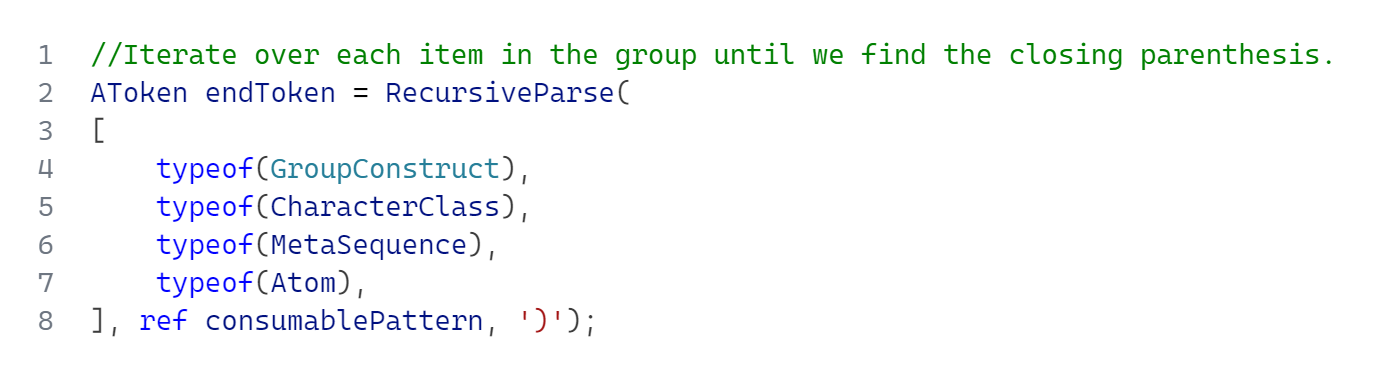
\includegraphics[width=\linewidth, height=0.3\textheight, keepaspectratio]{Figures/GroupConstructRecursiveParse.png}
    \end{subfigure}
    \begin{subfigure}[b]{0.5\textwidth}
        \caption{Recursive Token Parser}
        \label{fig:AToken_RecursiveParse}
        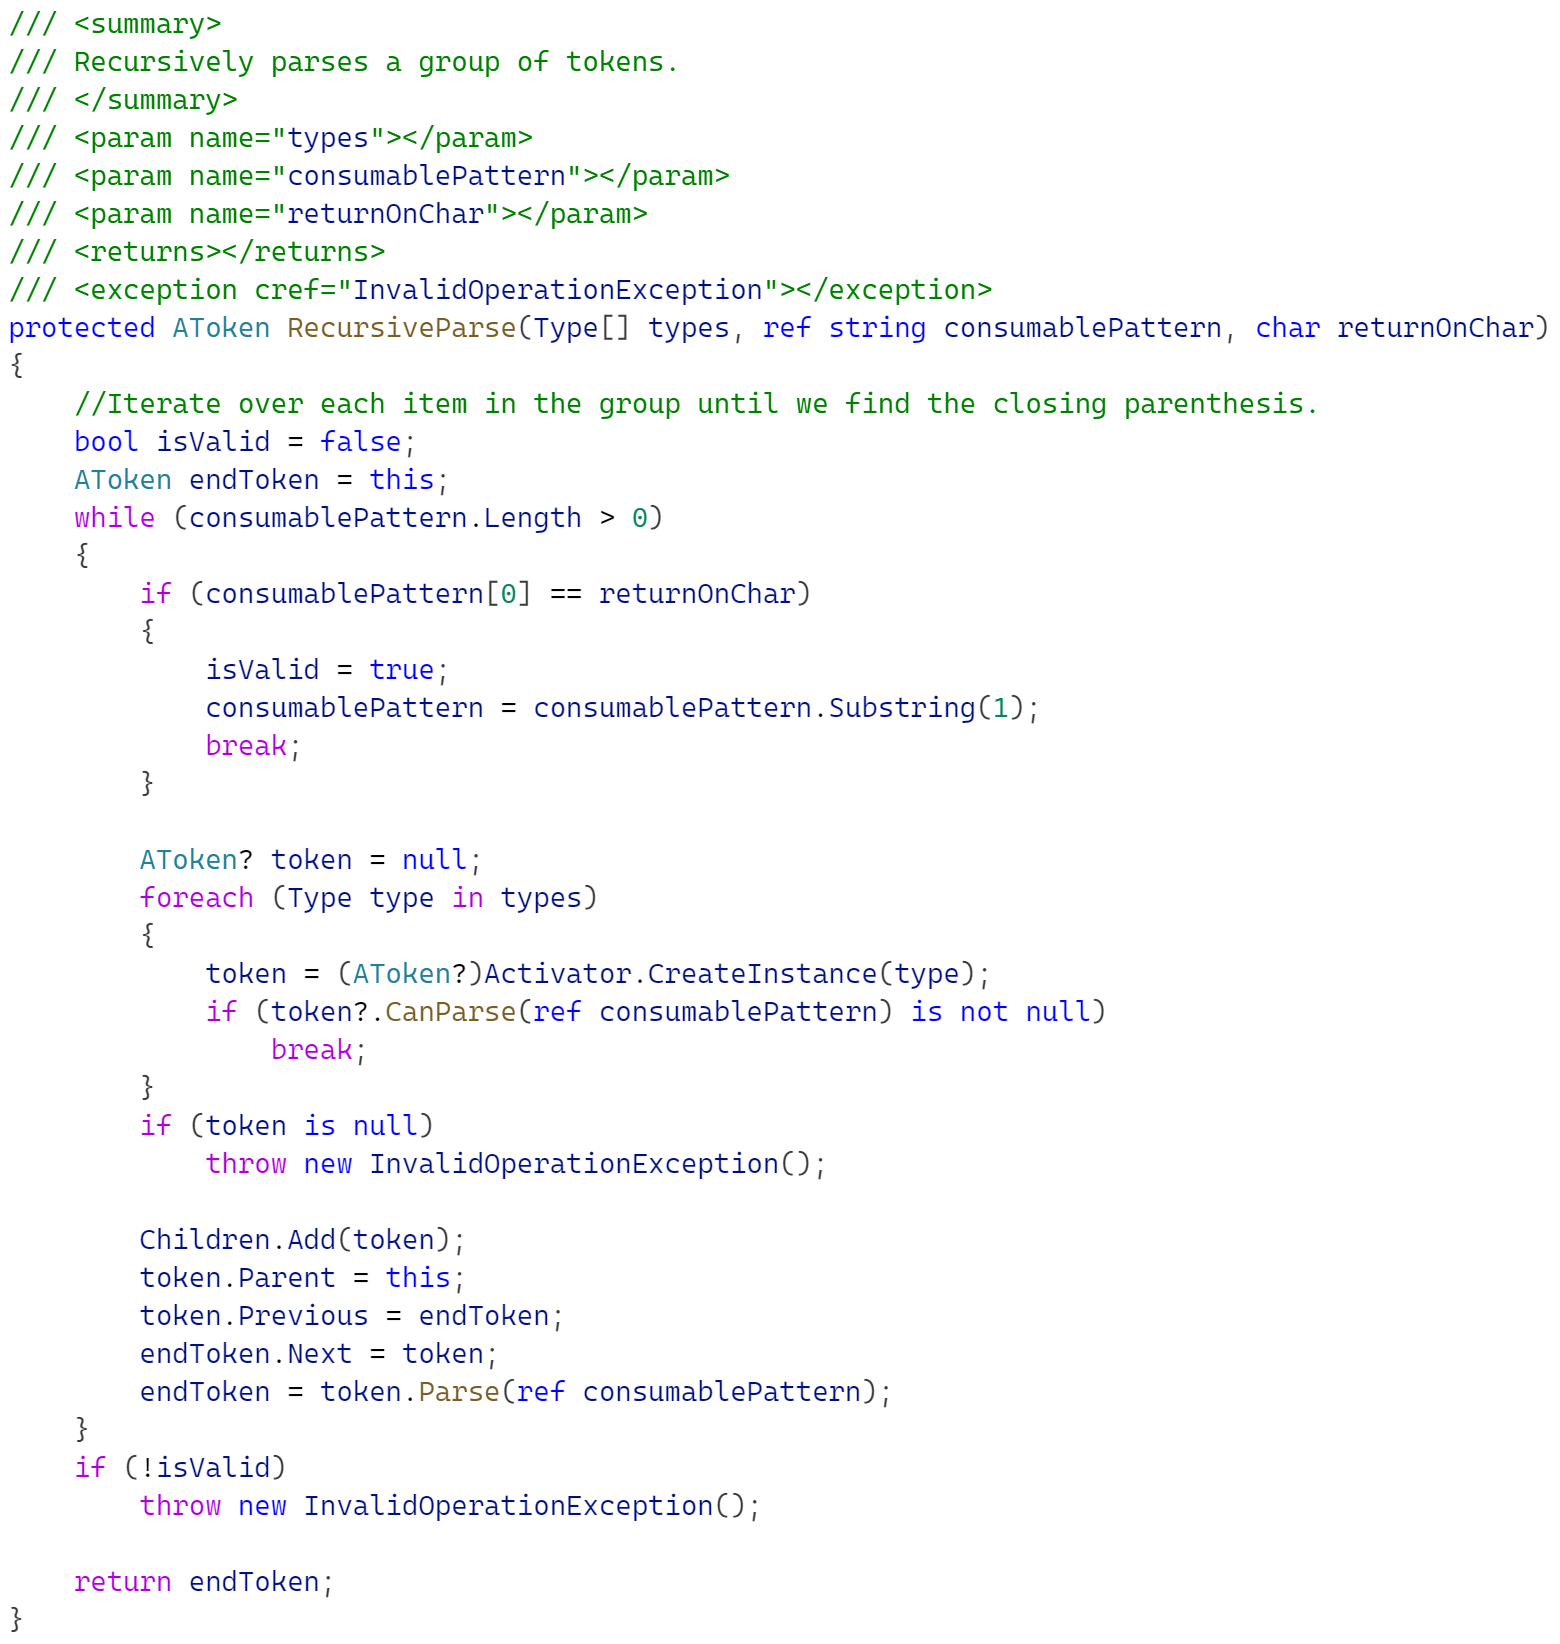
\includegraphics[width=\linewidth, height=\textheight, keepaspectratio]{Figures/AToken_RecursiveParse.png}
    \end{subfigure}
\end{wrapfigure}

The parse method is responsible for converting a pattern into a tree structure of tokens. Every token class has a different implementation of this method, for example, the group construct class will first check the construct type which could be for example a positive lookbehind. After this the helper, recursive parse method is called to parse the children within the group construct. This recursive parse method takes three parameters: a list of valid child tokens, a consumable pattern to parse, and a closing token to look for, the method will then proceed to consume the pattern and parse tokens (see figure \ref{fig:AToken_RecursiveParse}). For any valid tokens found a new instance of that token class is constructed and the parse method on that child will be called. After the child token has been parsed, the child tokens parent gets updated to the calling contexts token, the previous token of the child is set to the last token in the parent's children list, and the child token is added to the parent's children list. The method will then continue to consume the pattern until the closing token is found. If the closing token is not found, the method will throw an exception due to the pattern being invalid. If the closing token is found, the method will return the parsed tokens. The parse method is called recursively on the root token to parse the entire pattern into a tree structure of tokens.

\subsubsubsection{Input conversion}
The second part of the regex engine is the convert function. This function will attempt to convert an input string to conform to the pattern that the object was initialized with.
% TODO: Show the configuration options and what effect they have on the conversion.
Along with the input string, various options can be passed to the convert function to allow for fine-tuning of the conversion process. These options exist as there may be scenarios where certain parts of the pattern need to behave differently, for example, for literal tokens, the user may want to remove mismatched tokens or replace them with a valid token.
For the scenario of renaming code objects, we more often than not want to remove mismatched literals with a blank. To provide an example of this, if we want to conform the input \texttt{\_\_my\_variable} to the pattern \texttt{([A-Z][a-z]+)+}, it should produce a desired output of \texttt{MyVariable}. If mismatched tokens were not dropped the algorithm would fail to conform to the pattern as the pattern provides no way to match the literal characters \texttt{\_\_} to the pattern. By dropping these mismatched characters, the algorithm effectively ignores them from the output and matches where it can on valid tokens, producing an output of \texttt{MyVariable}.
% TODO: Show the detailed workings of the conversion process.

\subsubsubsection{Output validation}
The final part of the regex engine is the match function. This function will validate wether the result from the conform function matches the pattern that the object was initialized with. Usually this function does not need to be called as the conform method will either succeed of fail. The method exists as a validation step to ensure that the output is correct for the provided pattern using the custom regex engine algorithm as it may possibly differ from the standard C\# regex engine.
% TODO: Show edge cases where this may be used.
